\documentclass[11pt,letterpaper]{article}
\usepackage[lmargin=1in,rmargin=1in,tmargin=1in,bmargin=1in]{geometry}
\usepackage{../style/homework}
\usepackage{../style/commands}
\setbool{quotetype}{true} % True: Side; False: Under
\setbool{hideans}{true} % Student: True; Instructor: False

% -------------------
% Content
% -------------------
\begin{document}

\homework{14: Due 04/26}{Geometry is the science of correct reasoning on incorrect figures}{George P\'olya}

% Problem 1
\problem{10} Consider the right triangles shown below. Find the value of $d$.
	\[
	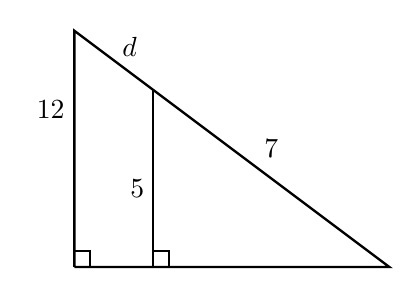
\begin{tikzpicture}
	\draw[line width=0.03cm] (0,0) -- (0,3) -- (4,0) -- (0,0);
	\draw[line width=0.03cm] (1,0) -- (1,2.25);
	\draw[line width=0.03cm] (0,0.2) -- (0.2,0.2) -- (0.2,0);
	\draw[line width=0.03cm] (1,0.2) -- (1.2,0.2) -- (1.2,0);
	\node at (-0.3,2) {$12$};
	\node at (0.8,1) {$5$};
	\node at (0.7,2.8) {$d$};
	\node at (2.5,1.5) {$7$};
	\end{tikzpicture}
	\]



\newpage



% Problem 2
\problem{10} For the triangles $\Delta ABC$ and $\Delta DEF$, shown below, assume that $\Delta ABC \sim \Delta DEF$. Find the missing sides of $\Delta DEF$. 
	\[
	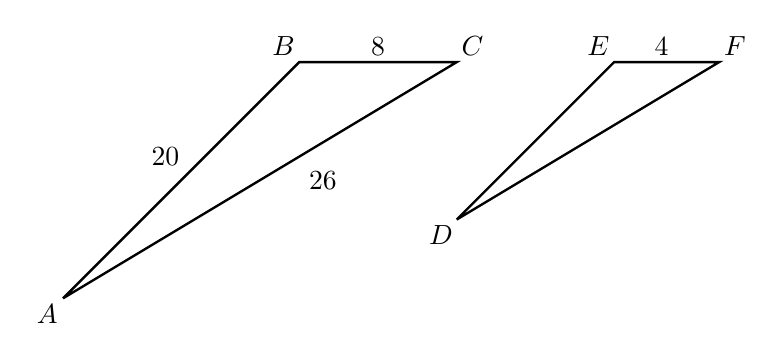
\begin{tikzpicture}
	\node at (-3.2,-3.2) {$A$};
	\node at (-0.2,0.2) {$B$};
	\node at (2.2,0.2) {$C$};
	\node at (-1.7,-1.2) {$20$};
	\node at (1,0.2) {$8$};
	\node at (0.3,-1.5) {$26$};
	\draw[line width=0.03cm] (-3,-3) -- (0,0) -- (2,0) -- (-3,-3);
	
	\tikzset{shift={(4,0)}}
	
	\node at (-2.2,-2.2) {$D$};
	\node at (-0.2,0.2) {$E$};
	\node at (4/3+0.2,0.2) {$F$};
	\node at (0.6,0.2) {$4$};
	\draw[line width=0.03cm] (-2,-2) -- (0,0) -- (4/3,0) -- (-2,-2);
	\end{tikzpicture}
	\]



\newpage



% Problem 3
\problem{10} Consider the triangles shown below. \par
	\[
	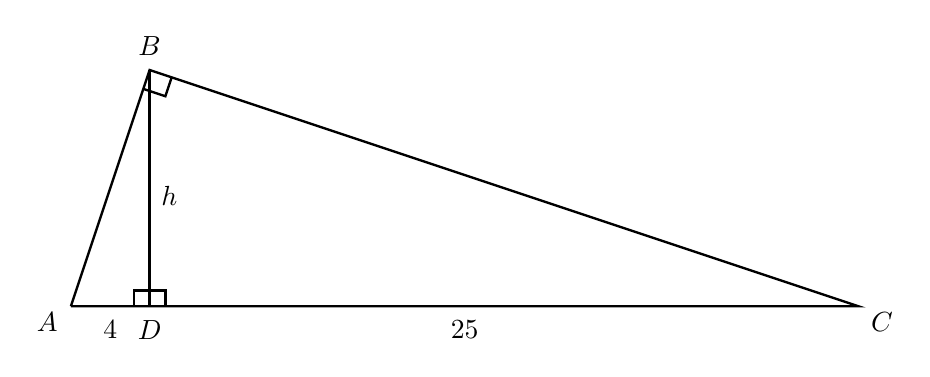
\begin{tikzpicture}
	\draw[line width=0.03cm] (0,0) -- (1,3) -- (10,0) -- (0,0);
	\draw[line width=0.03cm] (1,3) -- (1,0);
	\draw[line width=0.03cm] (0.8,0) -- (0.8,0.2) -- (1.2,0.2) -- (1.2,0);
	\draw[line width=0.03cm] (0.92,2.76) -- (1.2,2.666) -- (1.2802,2.9066);
	\node at (-0.3,-0.2) {$A$};
	\node at (1,3.3) {$B$};
	\node at (10.3,-0.2) {$C$};
	\node at (1,-0.3) {$D$};
	\node at (0.5,-0.3) {$4$};
	\node at (1.25,1.4) {$h$};
	\node at (5,-0.3) {$25$};
	\end{tikzpicture}
	\] \par

\begin{enumerate}[(a)]
\item Explain why $\Delta ADB \sim \Delta ABC$ and $\Delta BDC \sim \Delta ABC$. 
\item Does (a) imply that $\Delta ADB \sim BDC$? Explain. 
\item Find $h$. 
\end{enumerate}


\end{document}